\documentclass{article}
\usepackage{longtable}
\usepackage{multirow}
\usepackage{array}
\usepackage{graphicx}  % For inserting images
\usepackage{caption}   % For better caption formatting
\usepackage{float}     % To control figure placement
\usepackage{booktabs}
\usepackage{array}
\usepackage{epsfig}
\usepackage{float}  % Allows better figure placement
\usepackage{tabularx} 

\graphicspath{{fig/}} % Set the directory where graphics are located



\title{Artifact}
\author{Eduardo Oliveira}
\date{\today}

\begin{document}

\maketitle

\section{Open Science Platform}

\subsection{Overview}

Traditional centralized systems often exhibit data silos, limited verifiability, and susceptibility to manipulation, impeding the openness and reliability of scientific practices. The decentralized model introduced in this work is designed to mitigate these challenges by enabling efficient data sharing, fostering collaboration, and enhancing the validation of research outputs, thereby strengthening reproducibility and transparency.

This chapter details the design and implementation of the Open Science Platform, a decentralized system that integrates blockchain, IPFS, and smart contracts to improve research reproducibility. By leveraging immutable records and decentralized storage, the platform ensures transparent and verifiable research artifact management. Additionally, extended services are incorporated to facilitate file indexing, metadata extraction, and search functionality. The proposed platform aligns with Open Science principles by providing verifiable and persistently traceable access to research artifacts.


\begin{figure}[htbp]
      \centering
      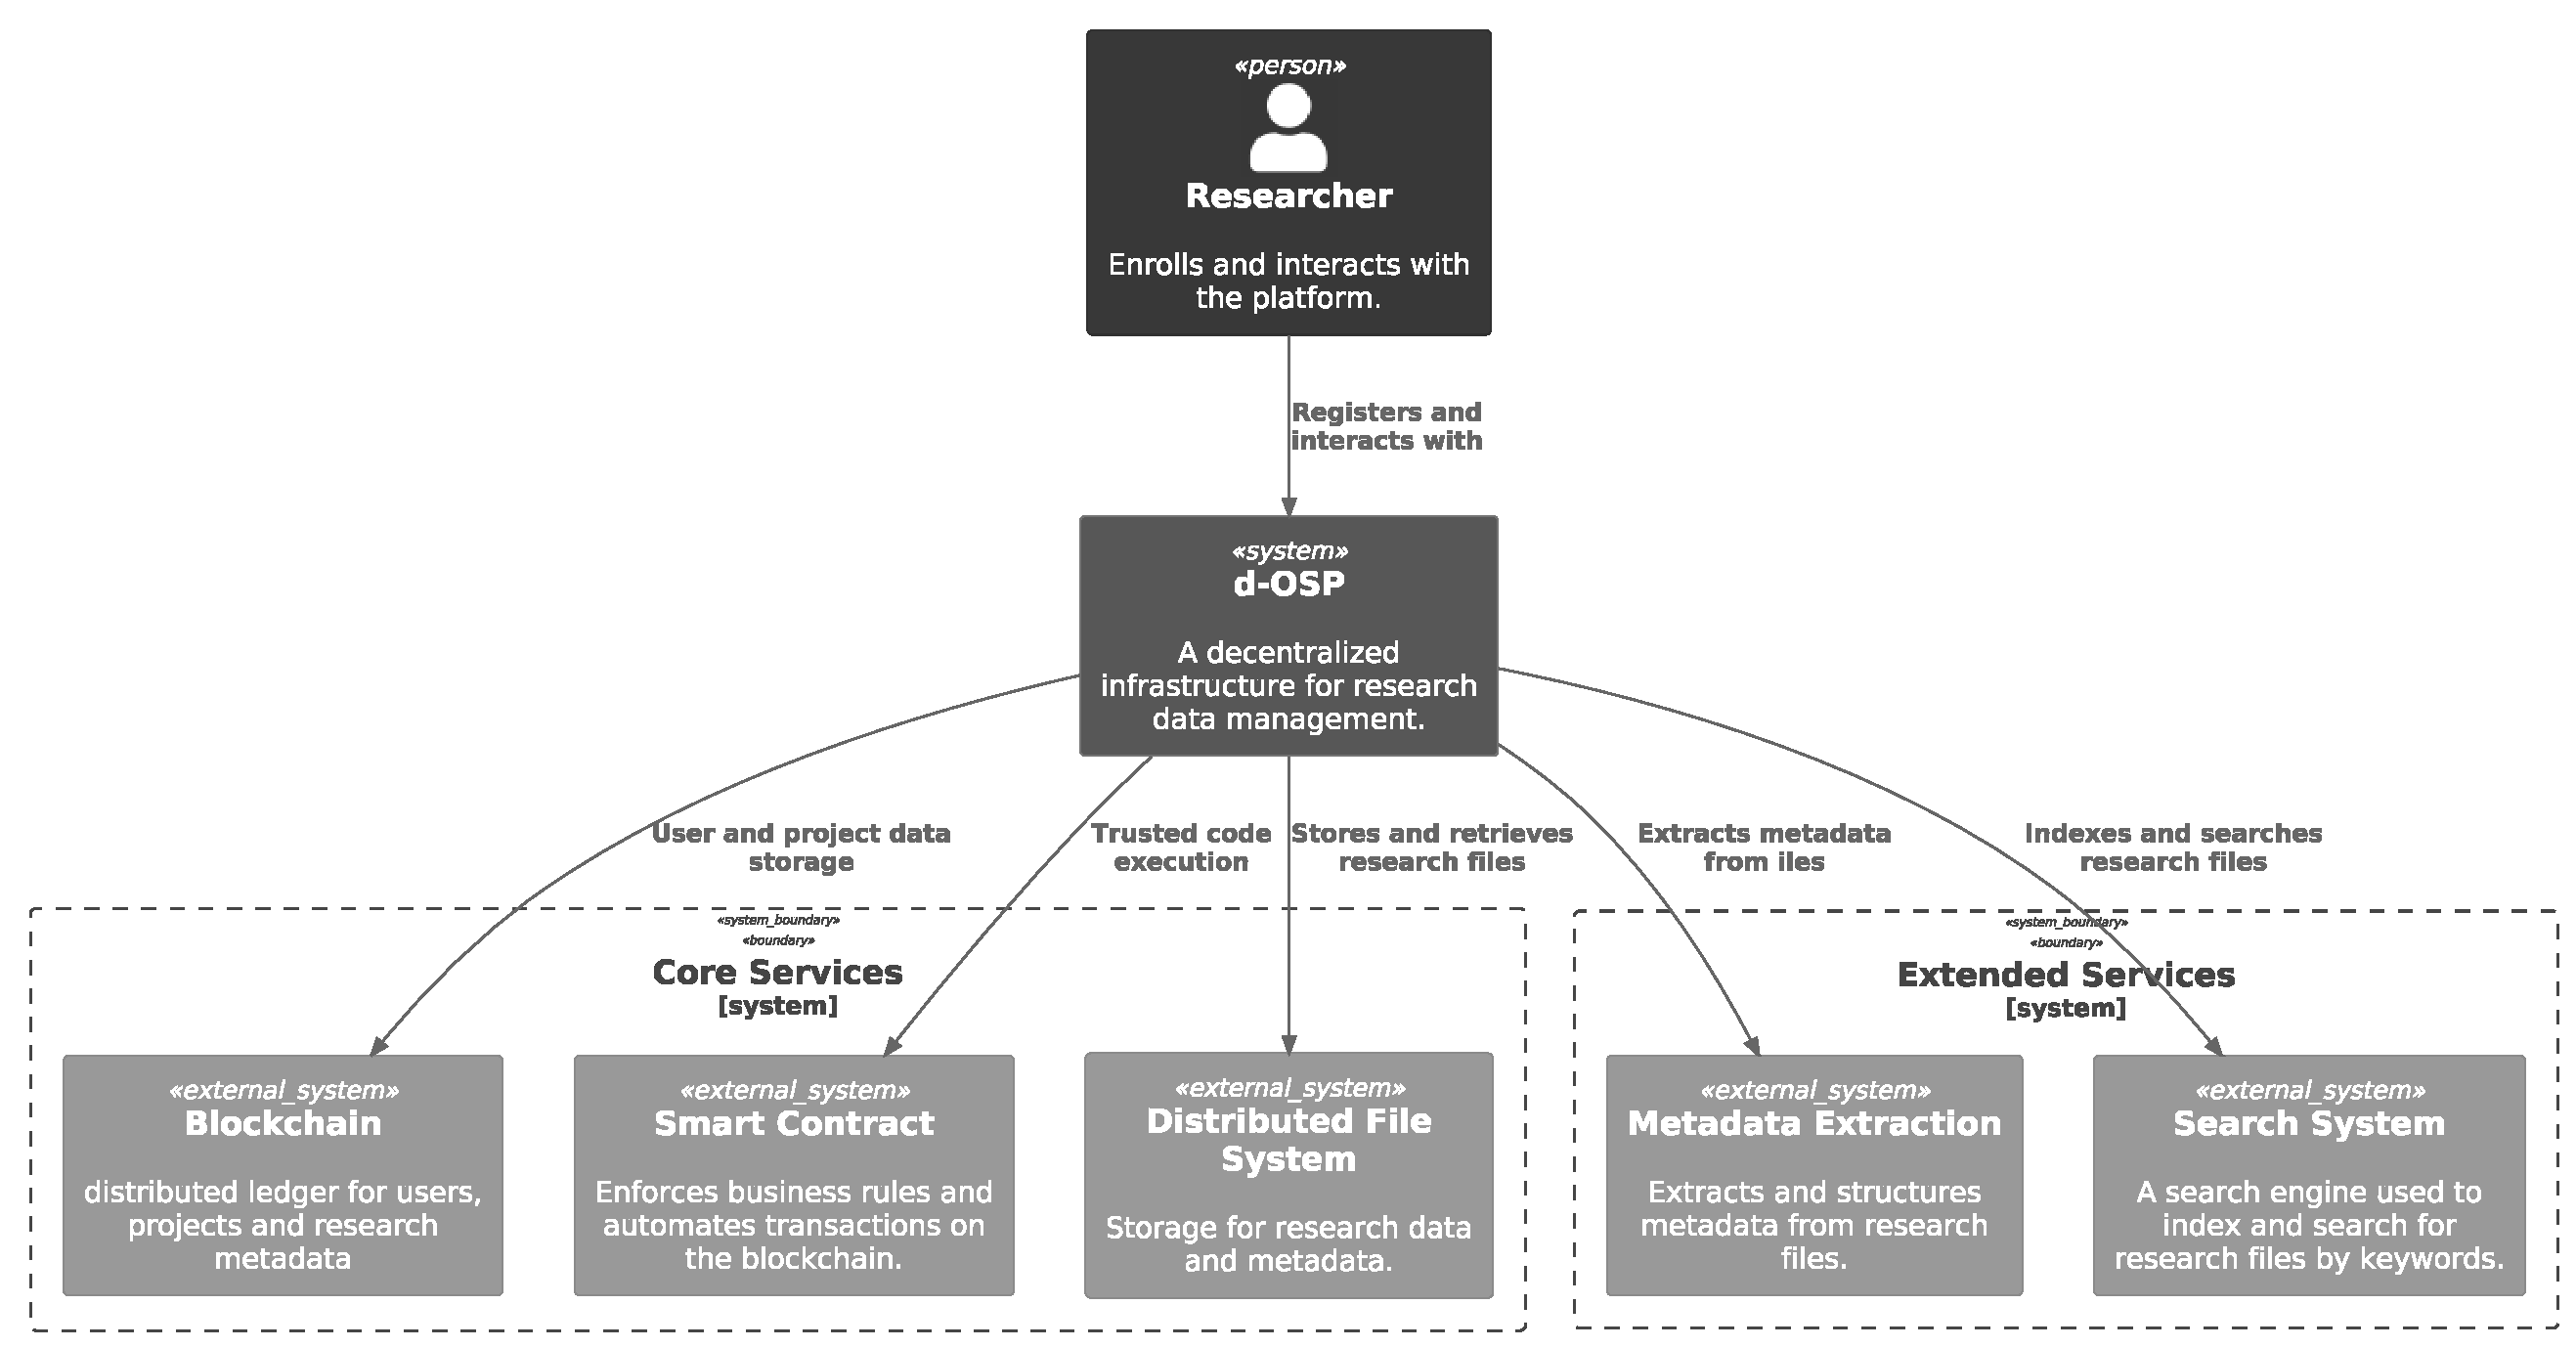
\includegraphics[width=0.98\textwidth, keepaspectratio]{c4_context_diagram}
      \caption{System context diagram for the Open Science Platform}
      \label{fig:c4_context_diagram}
\end{figure}



\subsection{Technology Stack}
The Open Science Platform is developed using a hybrid architecture that combines decentralized and off-chain technologies to ensure secure, traceable, and efficient data management.

\subsection{Core Services}

The core services of the Open Science Platform provide the fundamental infrastructure for secure and verifiable research artifact management.

\begin{itemize}
      \item \textbf{Hyperledger Iroha v1 Blockchain:} Acts as the core infrastructure for managing user and project accounts, recording transactions, and enforcing business rules via smart contracts to ensure secure and transparent data exchange.
      \item \textbf{InterPlanetary File System (IPFS):} Provides decentralized, tamper-proof storage for research artifacts and metadata, ensuring persistent and verifiable access to shared data.
\end{itemize}

\subsection{Extended Services}

The extended services enhance the platform's features by improving file and metadata processing.

\begin{itemize}
      \item \textbf{Apache Tika:} Extracts metadata from uploaded files, enhancing artifact organization and searchability.
      \item \textbf{Whoosh:} Facilitates efficient indexing and keyword-based search for stored artifacts.
\end{itemize}


\subsection{User Interface, integration and execution}

\begin{itemize}
      \item \textbf{Jupyter Notebooks (Python):} Powers the front-end interface, facilitating the automation and display of the execution steps. Blockchain interactions are managed via the Iroha v1 Python library, while communication with the IPFS network is handled through the HTTPS client library.
\end{itemize}

\begin{figure}[htbp]
      \centering
      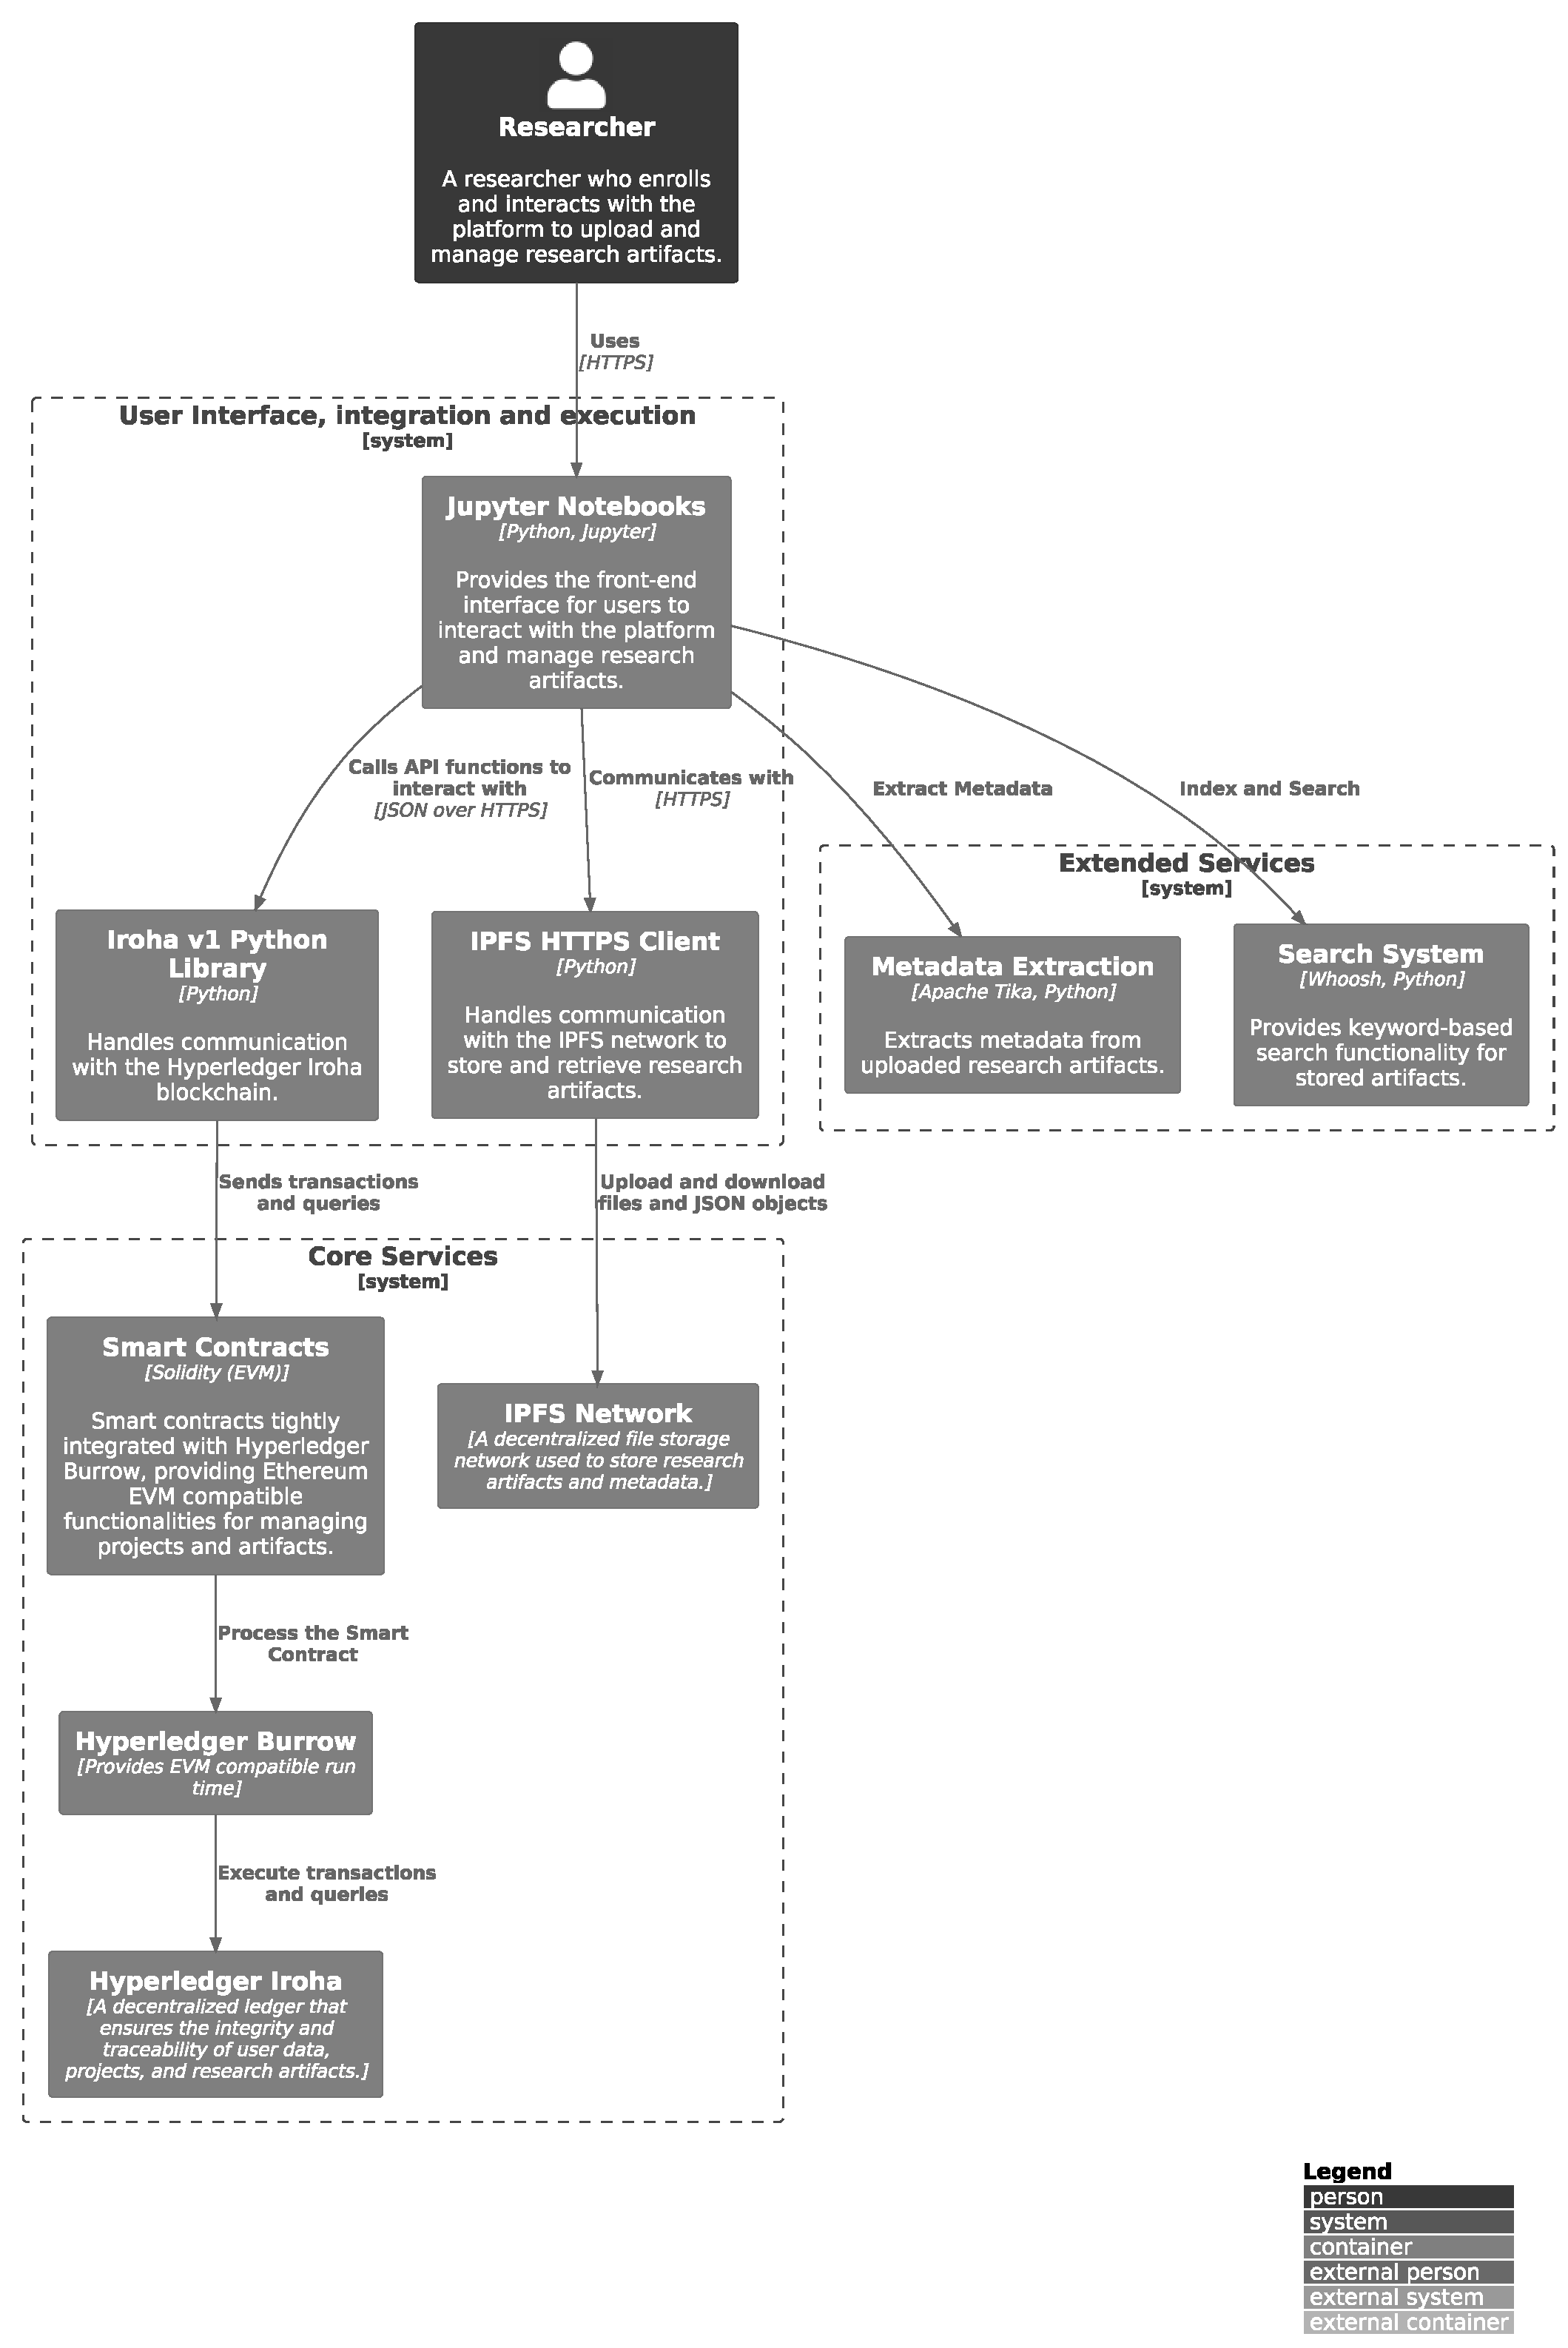
\includegraphics[width=0.98\textwidth, keepaspectratio]{c4_container_diagram}
      \caption{Container diagram for the Open Science Platform}
      \label{fig:c4_container_diagram}
\end{figure}


\subsection{System Components and Interactions in the Open Science Platform}

The Open Science Platform consists of multiple interconnected components, each serving a distinct role in ensuring secure, verifiable, and reproducible research data management. The primary components include Jupyter Server, the blockchain Hyperledger Iroha v1 and the InterPlanetary File System (IPFS). Each of these elements are encapsulated within a Docker container to provide modularity, ease of deployment and reproducibility.

\subsubsection{Jupyter Server}
The Jupyter Server acts as the primary interface for users interacting with the platform. This component provides a Python kernel for the execution environment that integrates the Iroha v1 Library, the IPFS HTTPS client, Apache Tika for metadata handling, and the Woosh Indexer and Search system. It enables users to:

\begin{itemize}
      \item Execute Python scripts to submit transactions and queries to the blockchain via smart contracts.
      \item Upload and retrieve files and metadata (JSON objects) stored in IPFS.
      \item Process and index research data using Apache Tika and Woosh for enhanced searchability.
      \item Access and visualize blockchain-stored metadata for Open Science applications.
\end{itemize}

\subsubsection{Blockchain}
The blockchain runs based on a Hyperledger Iroha v1 network and acts as a distributed ledger for recording transactions. It ensures immutability, transparency, and verifiability of stored research metadata. This component:
\begin{itemize}
      \item Receives transactions from the Jupyter Server via a gRPC API.
      \item Stores metadata references, ensuring that uploaded research artifacts can be authenticated.
      \item Interacts with PostgreSQL for structured storage of blockchain metadata.
      \item Supports smart contracts through the integration of Hyperledger Burrow, which provides a modular blockchain client with a permissioned smart contract interpreter partially developed to the specification of the Ethereum Virtual Machine (EVM).

\end{itemize}

\subsubsection{Storage}
The InterPlanetary File System (IPFS) is a decentralized storage solution that manages the research outputs. This component:
\begin{itemize}
      \item Stores digital research artifacts in a content-addressed manner.
      \item Allows the Jupyter Server to upload and retrieve files via an HTTPS API.
      \item Ensures long-term availability of scientific data through distributed storage principles.
\end{itemize}


\subsubsection{Relational Database (PostgreSQL)}
The PostgreSQL database provides structured storage for blockchain-related data. It is used exclusively and managed by Iroha v1 to:
\begin{itemize}
      \item Maintain an efficient and queryable record of transactions.
      \item Ensure that research metadata stored on the blockchain can be retrieved and verified.
      \item Support blockchain operations requiring fast access to structured data.
\end{itemize}

\subsubsection{Component Interactions}
The components interact in aseamless and decentralized manner:
\begin{enumerate}
      \item \textbf{User Interaction}: The user submits transactions, uploads files, and queries research data through the Jupyter Server.
      \item \textbf{Blockchain Transactions}: Jupyter Server sends and retrieves research metadata to the Iroha blockchain via gRPC API.
      \item \textbf{Metadata Storage}: Iroha stores data in the PostgreSQL database for efficient retrieval.
      \item \textbf{Decentralized Storage}: Research artifacts are stored in IPFS, with their unique file identifiers recorded on the blockchain.
      \item \textbf{File Retrieval}: Users can retrieve files from IPFS using their content identifiers (CID), ensuring authenticity and reproducibility.
\end{enumerate}

This architecture guarantees trustworthy and reproducible scientific research by leveraging blockchain for integrity, IPFS for decentralized storage, and Jupyter as an accessible research environment.


\begin{figure}[htbp]
      \centering
      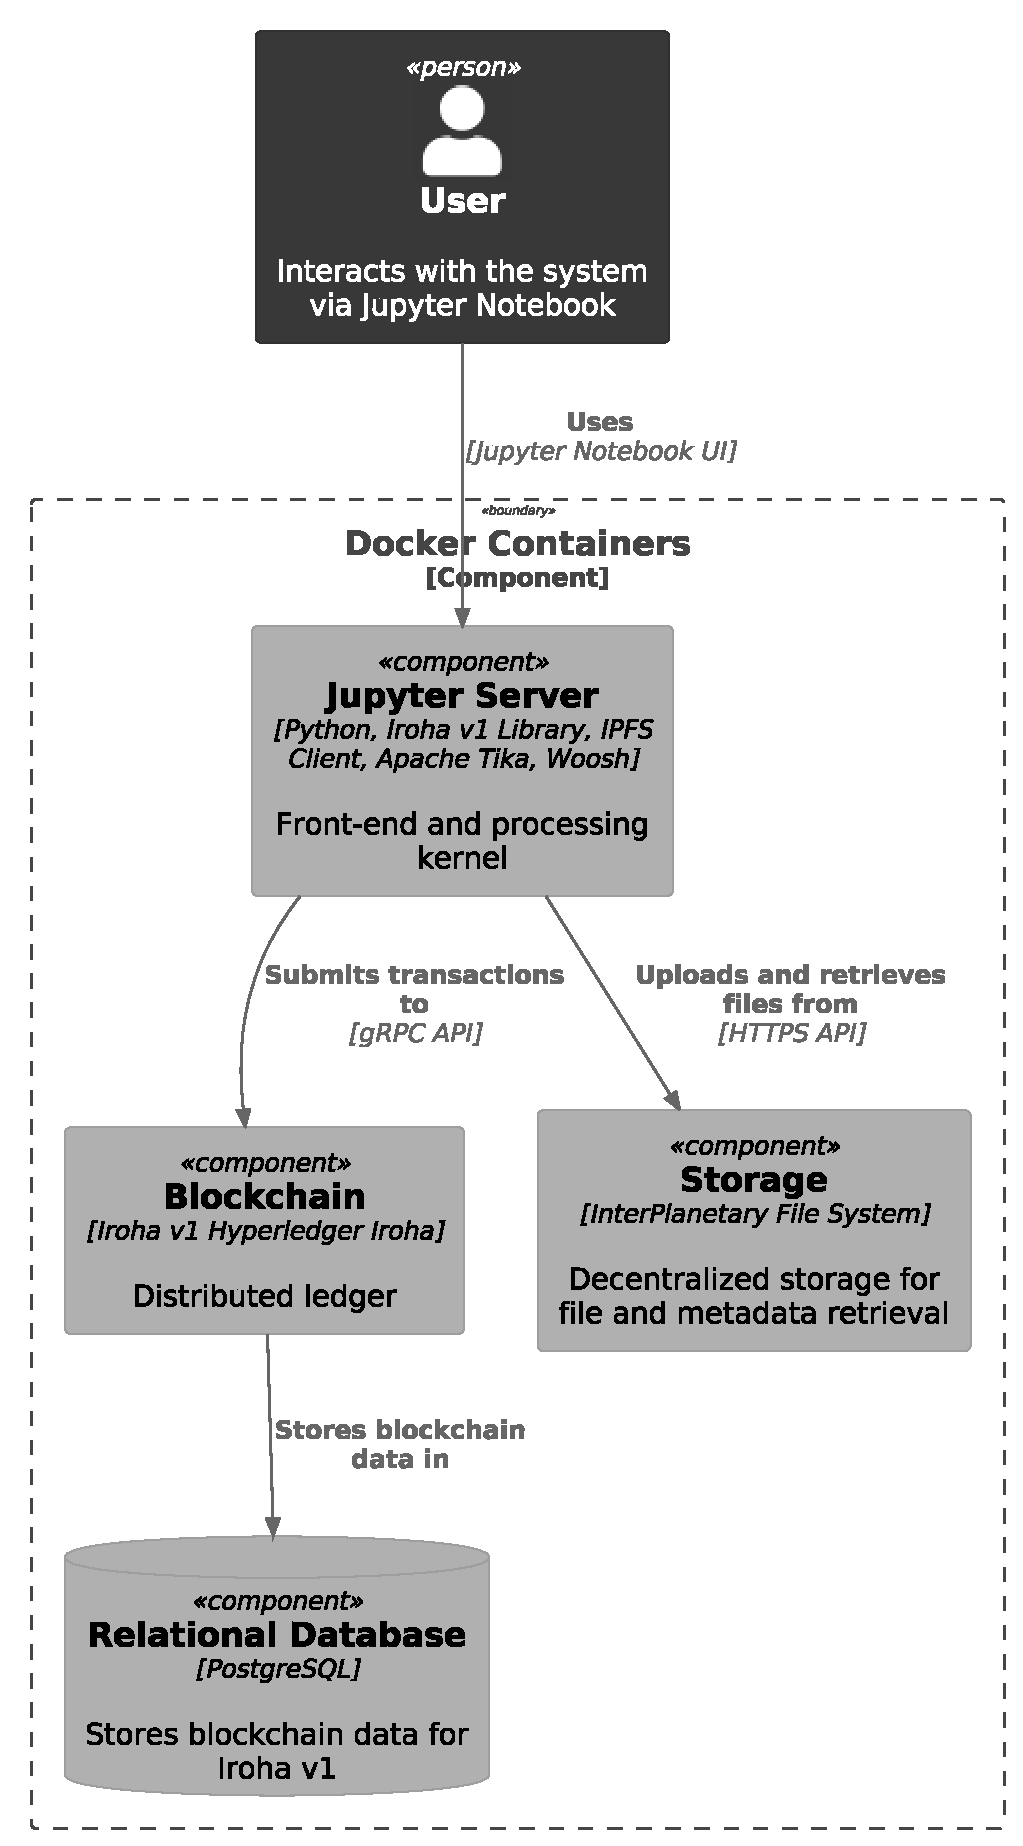
\includegraphics[width=0.98\textwidth, keepaspectratio]{c4_component_diagram.eps}
      \caption{Componentdiagram for the Open Science Platform}
      \label{fig:c4_component_diagram}
\end{figure}




\subsection{Platform Operations}
The platform supports a set of core operations that regulate user interactions with projects and data management.

\begin{itemize}
      \item \textbf{User Self-Enrollment} – A user self-enrolls on the platform by providing a private key that complies with the ED25519 or SHA-3 standards and identity information, including full name, institution, email, ORCID, and role. An account is created for the user in the blockchain. All data provided in the enrollment is structured in key/value pairs into a JSON object and uploaded to IPFS, with the corresponding Content Identifier (CID) recorded on the blockchain attributes of the user account.

      \item \textbf{Project Registration} – Users can register a project by specifying a descriptive name, an abstract, relevant keywords, start and end dates, funding agency, and location. Upon registration, a blockchain account is created. This data is structured in key/value pairs into a JSON object and uploaded to IPFS, with the corresponding Content Identifier (CID) recorded on the blockchain attributes of the project account.


      \item \textbf{User and Project Accounts Linkage} – Once both user and project accounts are created, the system updates their attributes to establish a bidirectional association. This ensures that querying a user account reveals linked project accounts, and vice versa, facilitating traceability and efficient project management.
\end{itemize}


\begin{figure}[htbp]
      \centering
      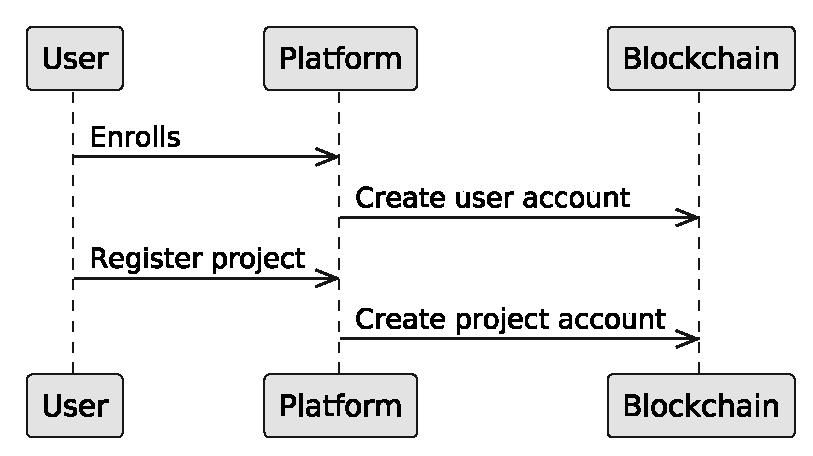
\includegraphics[width=0.98\textwidth, keepaspectratio]{c4_platform_operations_1}
      \caption{User enrollment and project registering for the Open Science Platform}
      \label{fig:c4_operations_diagram}
\end{figure}


\subsection{Artifact Management}

\begin{itemize}
      \item \textbf{File Upload} – A user may upload research artifacts, including papers, datasets, and images. Each file is stored on IPFS, generating a unique Content Identifier (CID) that ensures traceability and integrity. The CID is then recorded on the blockchain attributes of the project, establishing a verifiable reference to the artifact.

      \item \textbf{Metadata Extraction and Storage} – After the upload,the file available metadata is extracted. The extracted metadata is structured in key/value pairs into a JSON object and uploaded to IPFS, with the corresponding Content Identifier (CID) recorded on the attributes of the project account in the blockchain, ensuring metadata provenance and verification.

      \item \textbf{Indexing} – To facilitate efficient retrieval, the system indexes the metadata of every uploaded file, including full text indexing for text based files.

      \item \textbf{Searching} – Users can perform keyword-based searches to locate relevant research artifacts, with search results displaying metadata details, including descriptions, subject and authorship.
\end{itemize}


\begin{figure}[htbp]
      \centering
      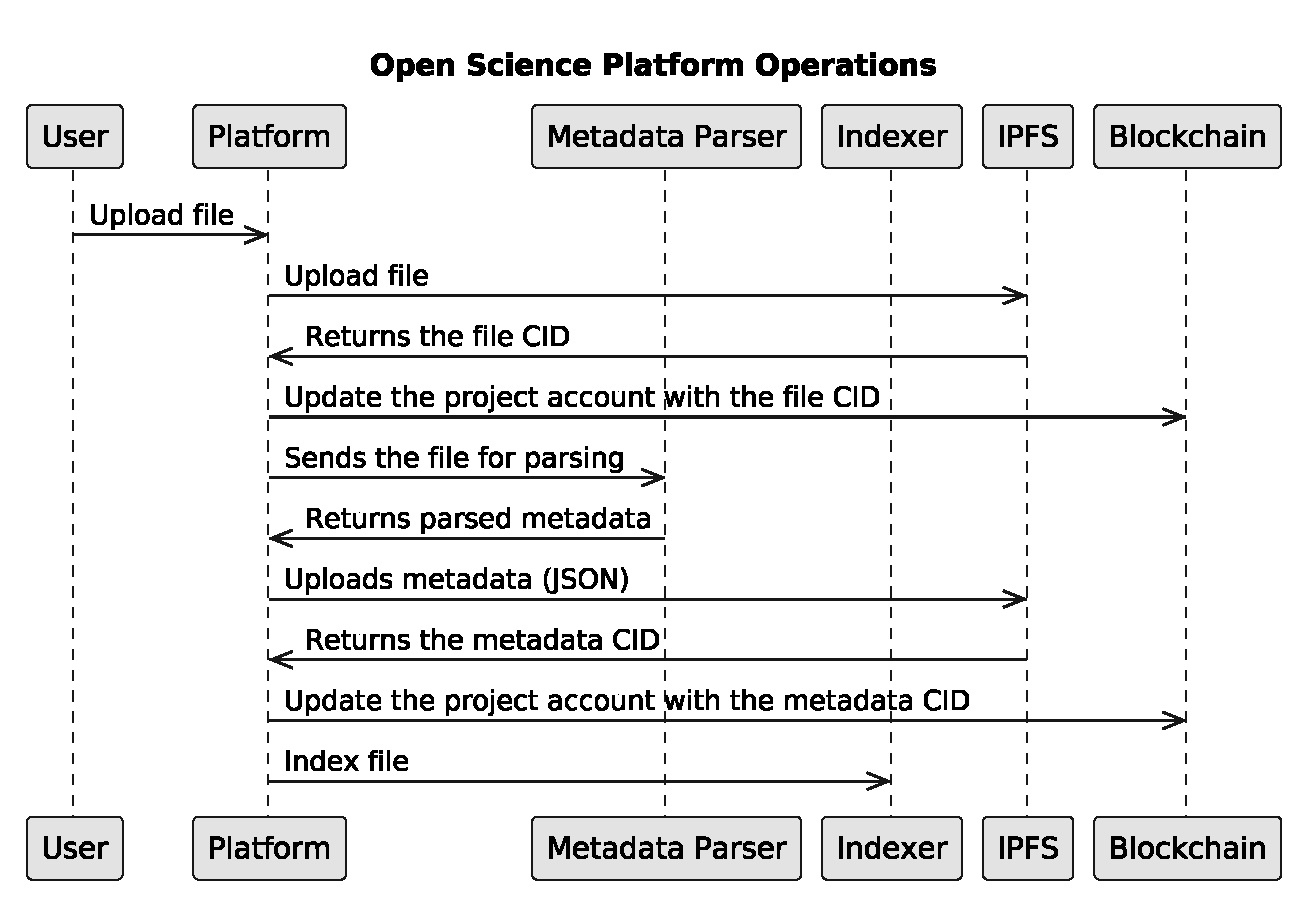
\includegraphics[width=0.98\textwidth, keepaspectratio]{c4_platform_operations_2}
      \caption{File operations diagram for the Open Science Platform}
      \label{fig:c4_file_operations_diagram}
\end{figure}


\begin{figure}[htbp]
      \centering
      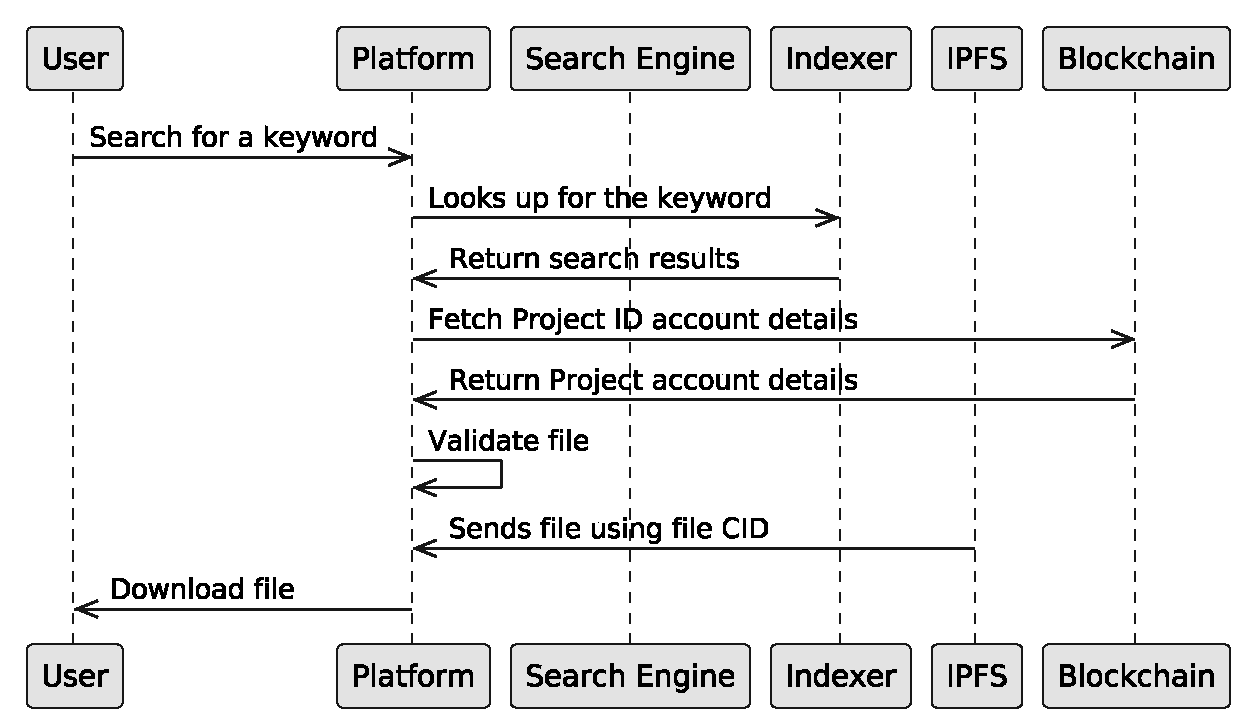
\includegraphics[width=0.98\textwidth, keepaspectratio]{c4_searching_and_validation.eps}
      \caption{keyword search, file validation and download}
      \label{fig:c4_keyword_search}
\end{figure}



\subsection{Validation and Download}

\begin{itemize}
      \item \textbf{File Validation} – To ensure data integrity and authenticity, the platform verifies whether the CID of a file stored on IPFS matches the CID recorded on the blockchain. A discrepancy between these identifiers signals potential tampering or corruption.

      \item \textbf{File Download} – The system retrieves and downloads validated files from IPFS to the user local file system for later usage.
\end{itemize}


\begin{figure}[htbp]
      \centering
      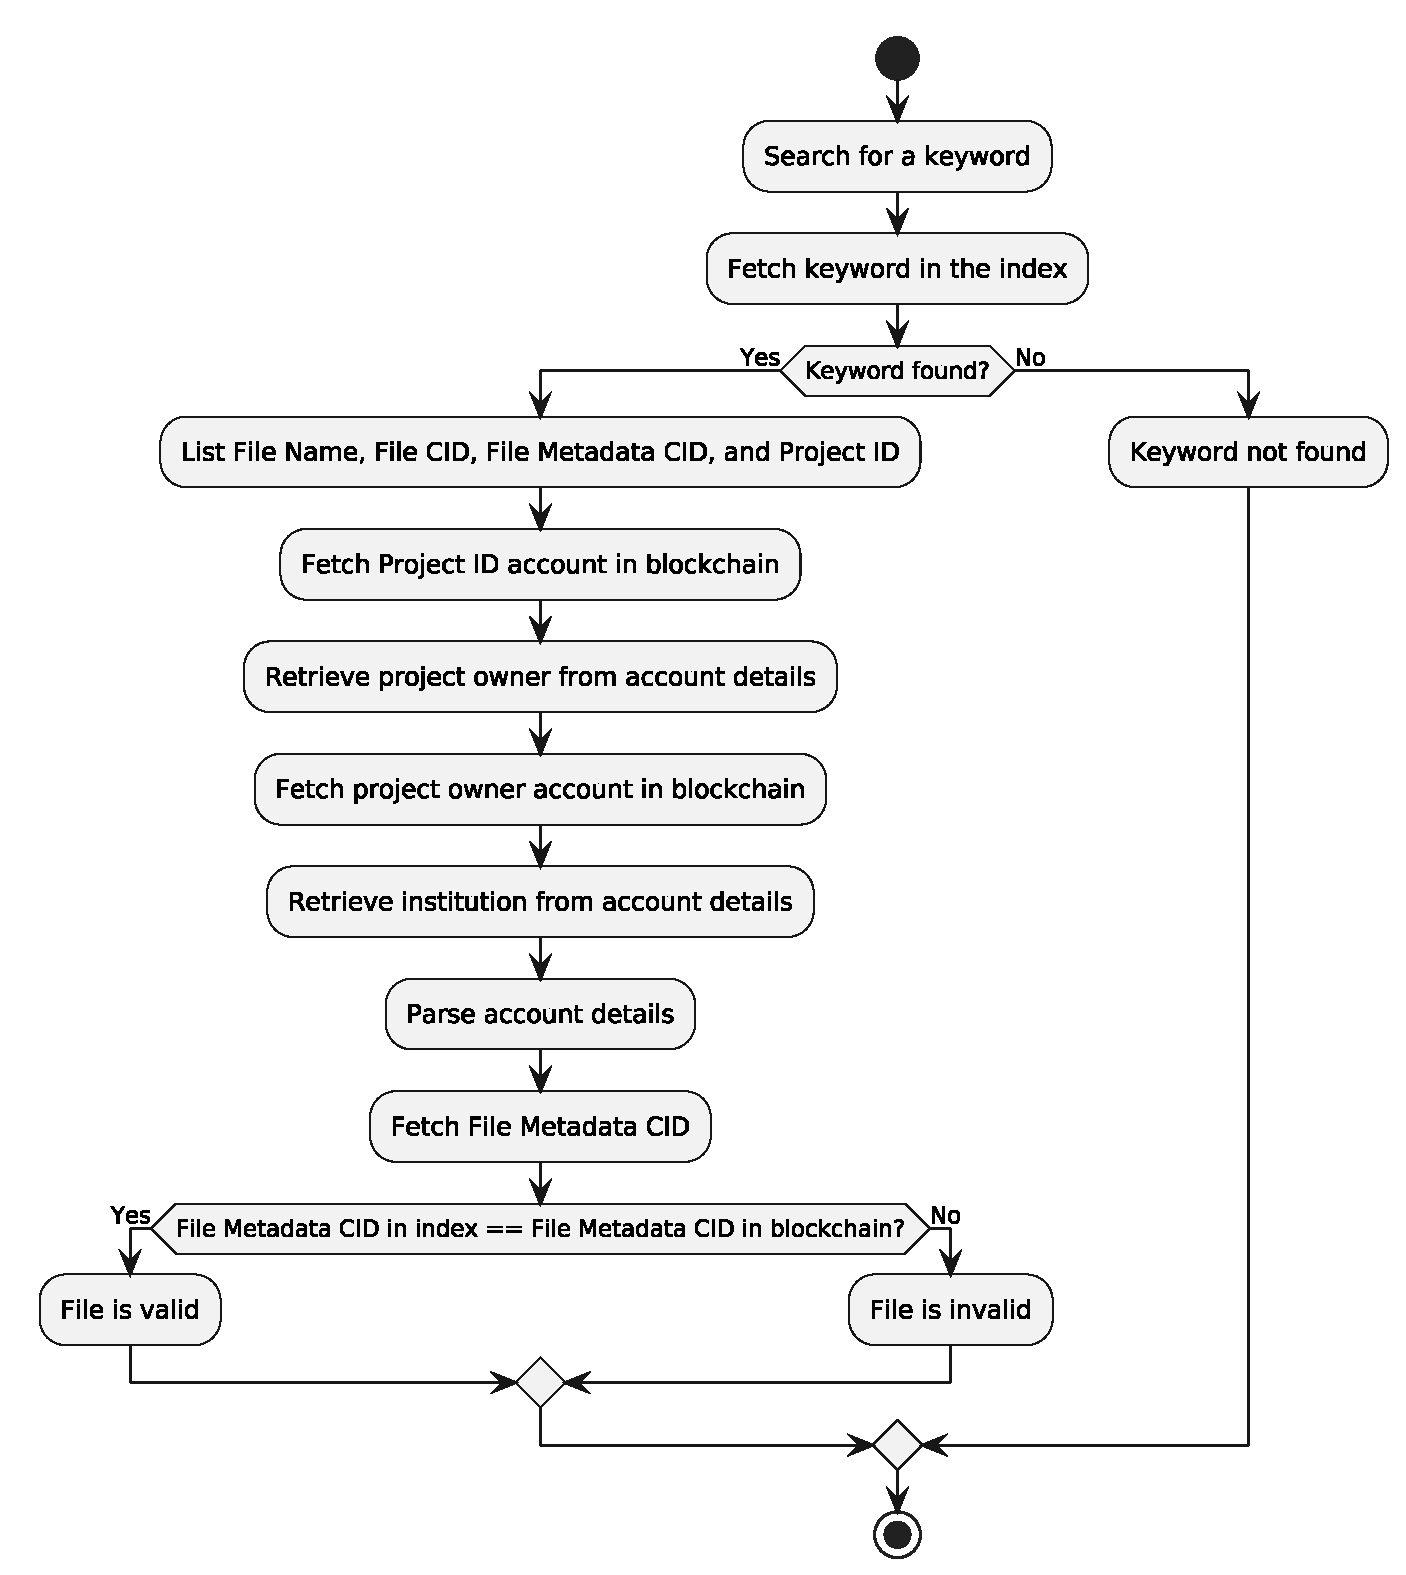
\includegraphics[width=0.98\textwidth, keepaspectratio]{keyword_and_file_validation.eps}
      \caption{File validation and download}
      \label{fig:c4_file_validation}
\end{figure}



\subsection{Data Model for the Open Science Platform}

The entity-relationship model for the Open Science Platform defines the logical structure of users and research projects, capturing the associations between these entities. The primary entities in this model are \texttt{User} and \texttt{Project}, which are connected through an ownership relationship.


\begin{figure}[htbp]
      \centering
      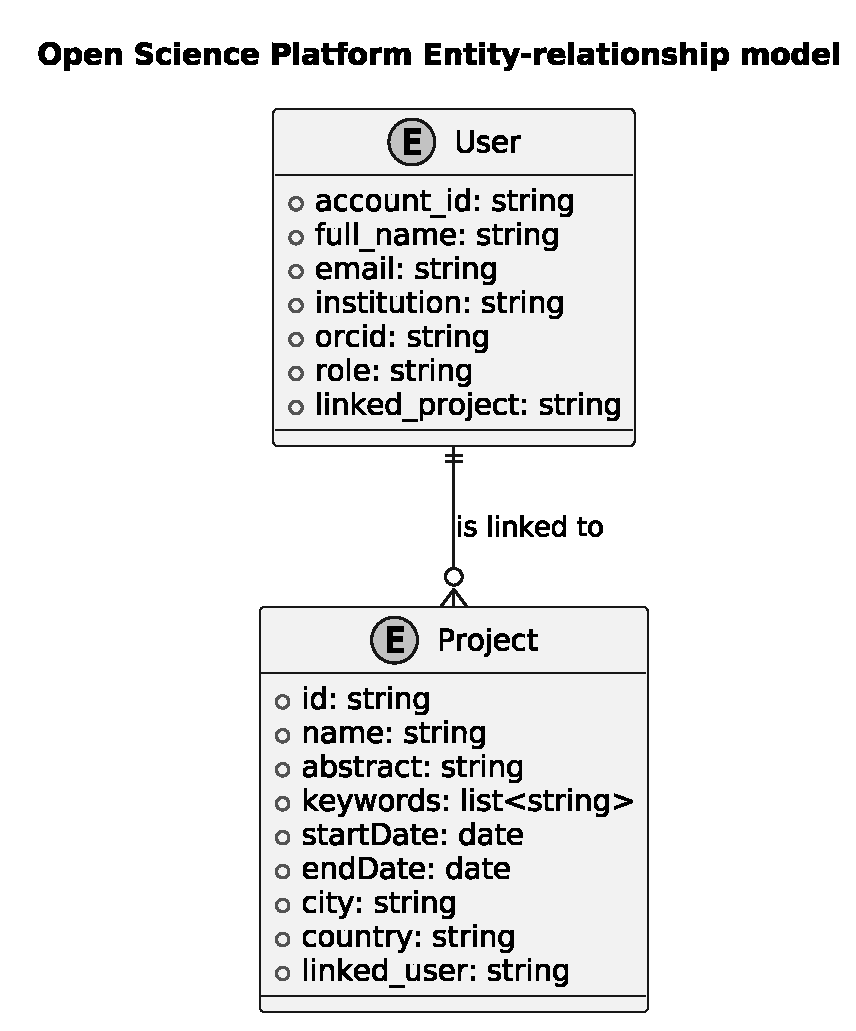
\includegraphics[width=0.98\textwidth, keepaspectratio]{entity_relationship_model.eps}
      \caption{Entity-relationship model for the Open Science Platform}
      \label{fig:er_model}
\end{figure}



\subsection{User Entity}
The \texttt{User} entity represents an individual interacting with the platform. Each user is uniquely identified by an account ID and has attributes that describe personal and institutional information. The attributes of the \texttt{User} entity are listed in Table \ref{tab:user_entity}.

\begin{table}[h]
      \centering
      \renewcommand{\arraystretch}{1.2}
      \caption{User Entity Attributes}
      \label{tab:user_entity}
      \begin{tabularx}{\textwidth}{|l|X|}
            \hline
            \textbf{Attribute}       & \textbf{Description}                              \\ \hline
            \texttt{account\_id}     & A unique identifier assigned to the user.         \\ \hline
            \texttt{full\_name}      & The complete name of the user.                    \\ \hline
            \texttt{email}           & The email address used for communication.         \\ \hline
            \texttt{institution}     & The organization to which the user is affiliated. \\ \hline
            \texttt{orcid}           & The Open Researcher and Contributor ID.           \\ \hline
            \texttt{role}            & The role of the user within the research project. \\ \hline
            \texttt{linked\_project} & The research project the user is assigned to.     \\ \hline
      \end{tabularx}
\end{table}


\subsection{Project Entity}
The \texttt{Project} entity represents a research project registered in the platform. It contains essential metadata to describe the project and facilitate discovery and collaboration. The attributes of the \texttt{Project} entity are listed in Table \ref{tab:project_entity}.

\begin{table}[h]
      \centering
      \renewcommand{\arraystretch}{1.2}
      \caption{Project Entity Attributes}
      \label{tab:project_entity}
      \begin{tabularx}{\textwidth}{|l|X|}
            \hline
            \textbf{Attribute}    & \textbf{Description}                                                \\ \hline
            \texttt{project\_id}  & A unique identifier assigned to the project.                        \\ \hline
            \texttt{name}         & The official name of the project.                                   \\ \hline
            \texttt{abstract}     & A brief summary outlining the research objectives.                  \\ \hline
            \texttt{keywords}     & A list of relevant keywords associated with the project.            \\ \hline
            \texttt{startDate}    & The date when the project officially begins.                        \\ \hline
            \texttt{endDate}      & The date when the project was concluded or is expected to conclude. \\ \hline
            \texttt{city}         & The city where the project is primarily conducted.                  \\ \hline
            \texttt{country}      & The country associated with the research project.                   \\ \hline
            \texttt{linked\_user} & The user linked to the project.                                     \\ \hline
      \end{tabularx}
\end{table}


\subsection{Ownership Relationship}
A \texttt{User} owns one or more \texttt{Project} entities, establishing a one-to-many relationship. This means that a single user can be responsible for multiple projects, but each project is owned by exactly one user. This relationship is crucial for managing project access, ensuring accountability, and maintaining provenance of research activities. This model ensures a structured representation of research projects and their associated users, supporting an organized approach to data management in the Open Science Platform.

\subsection{ Data Model for Hyperledger Iroha v1}

The entity-relationship (ER) model of Hyperledger Iroha defines the core entities, attributes, and relationships that facilitate role-based access control, asset management, and multi-signature security. While Iroha v1 includes a broader set of entities, this research focuses solely on the account and domain related classes and attributes.

\section{Core Entities and Their Attributes}
\subsection{Account Entity}
The \texttt{account} entity represents a user or system account registered on the blockchain. Table \ref{tab:account_attributes} lists its attributes.

\begin{table}[h]
      \centering
      \label{tab:account_entity}
      \renewcommand{\arraystretch}{1.2}
      \begin{tabularx}{\textwidth}{|l|X|}
            \hline
            \textbf{Attribute}   & \textbf{Description}                                            \\ \hline
            \texttt{account\_id} & Unique identifier of the account                                \\ \hline
            \texttt{domain\_id}  & Links the account to a specific domain                          \\ \hline
            \texttt{quorum}      & Required number of signatories for multi-signature transactions \\ \hline
            \texttt{data}        & Stores additional metadata in JSON format                       \\ \hline
      \end{tabularx}
\end{table}

\subsection{Domain Entity}
The \texttt{domain} entity organizes accounts within logical boundaries.A \texttt{domain} can have multiple \texttt{accounts}.

\begin{table}[h]
      \centering
      \label{tab:domain_entity}
      \renewcommand{\arraystretch}{1.2}
      \begin{tabularx}{\textwidth}{|l|X|}
            \hline
            \textbf{Attribute}     & \textbf{Description}                                    \\ \hline
            \texttt{domain\_id}    & Unique identifier for the domain                        \\ \hline
            \texttt{default\_role} & Default role assigned to accounts created in the domain \\ \hline
      \end{tabularx}
\end{table}


\begin{figure}[htbp]
      \centering
      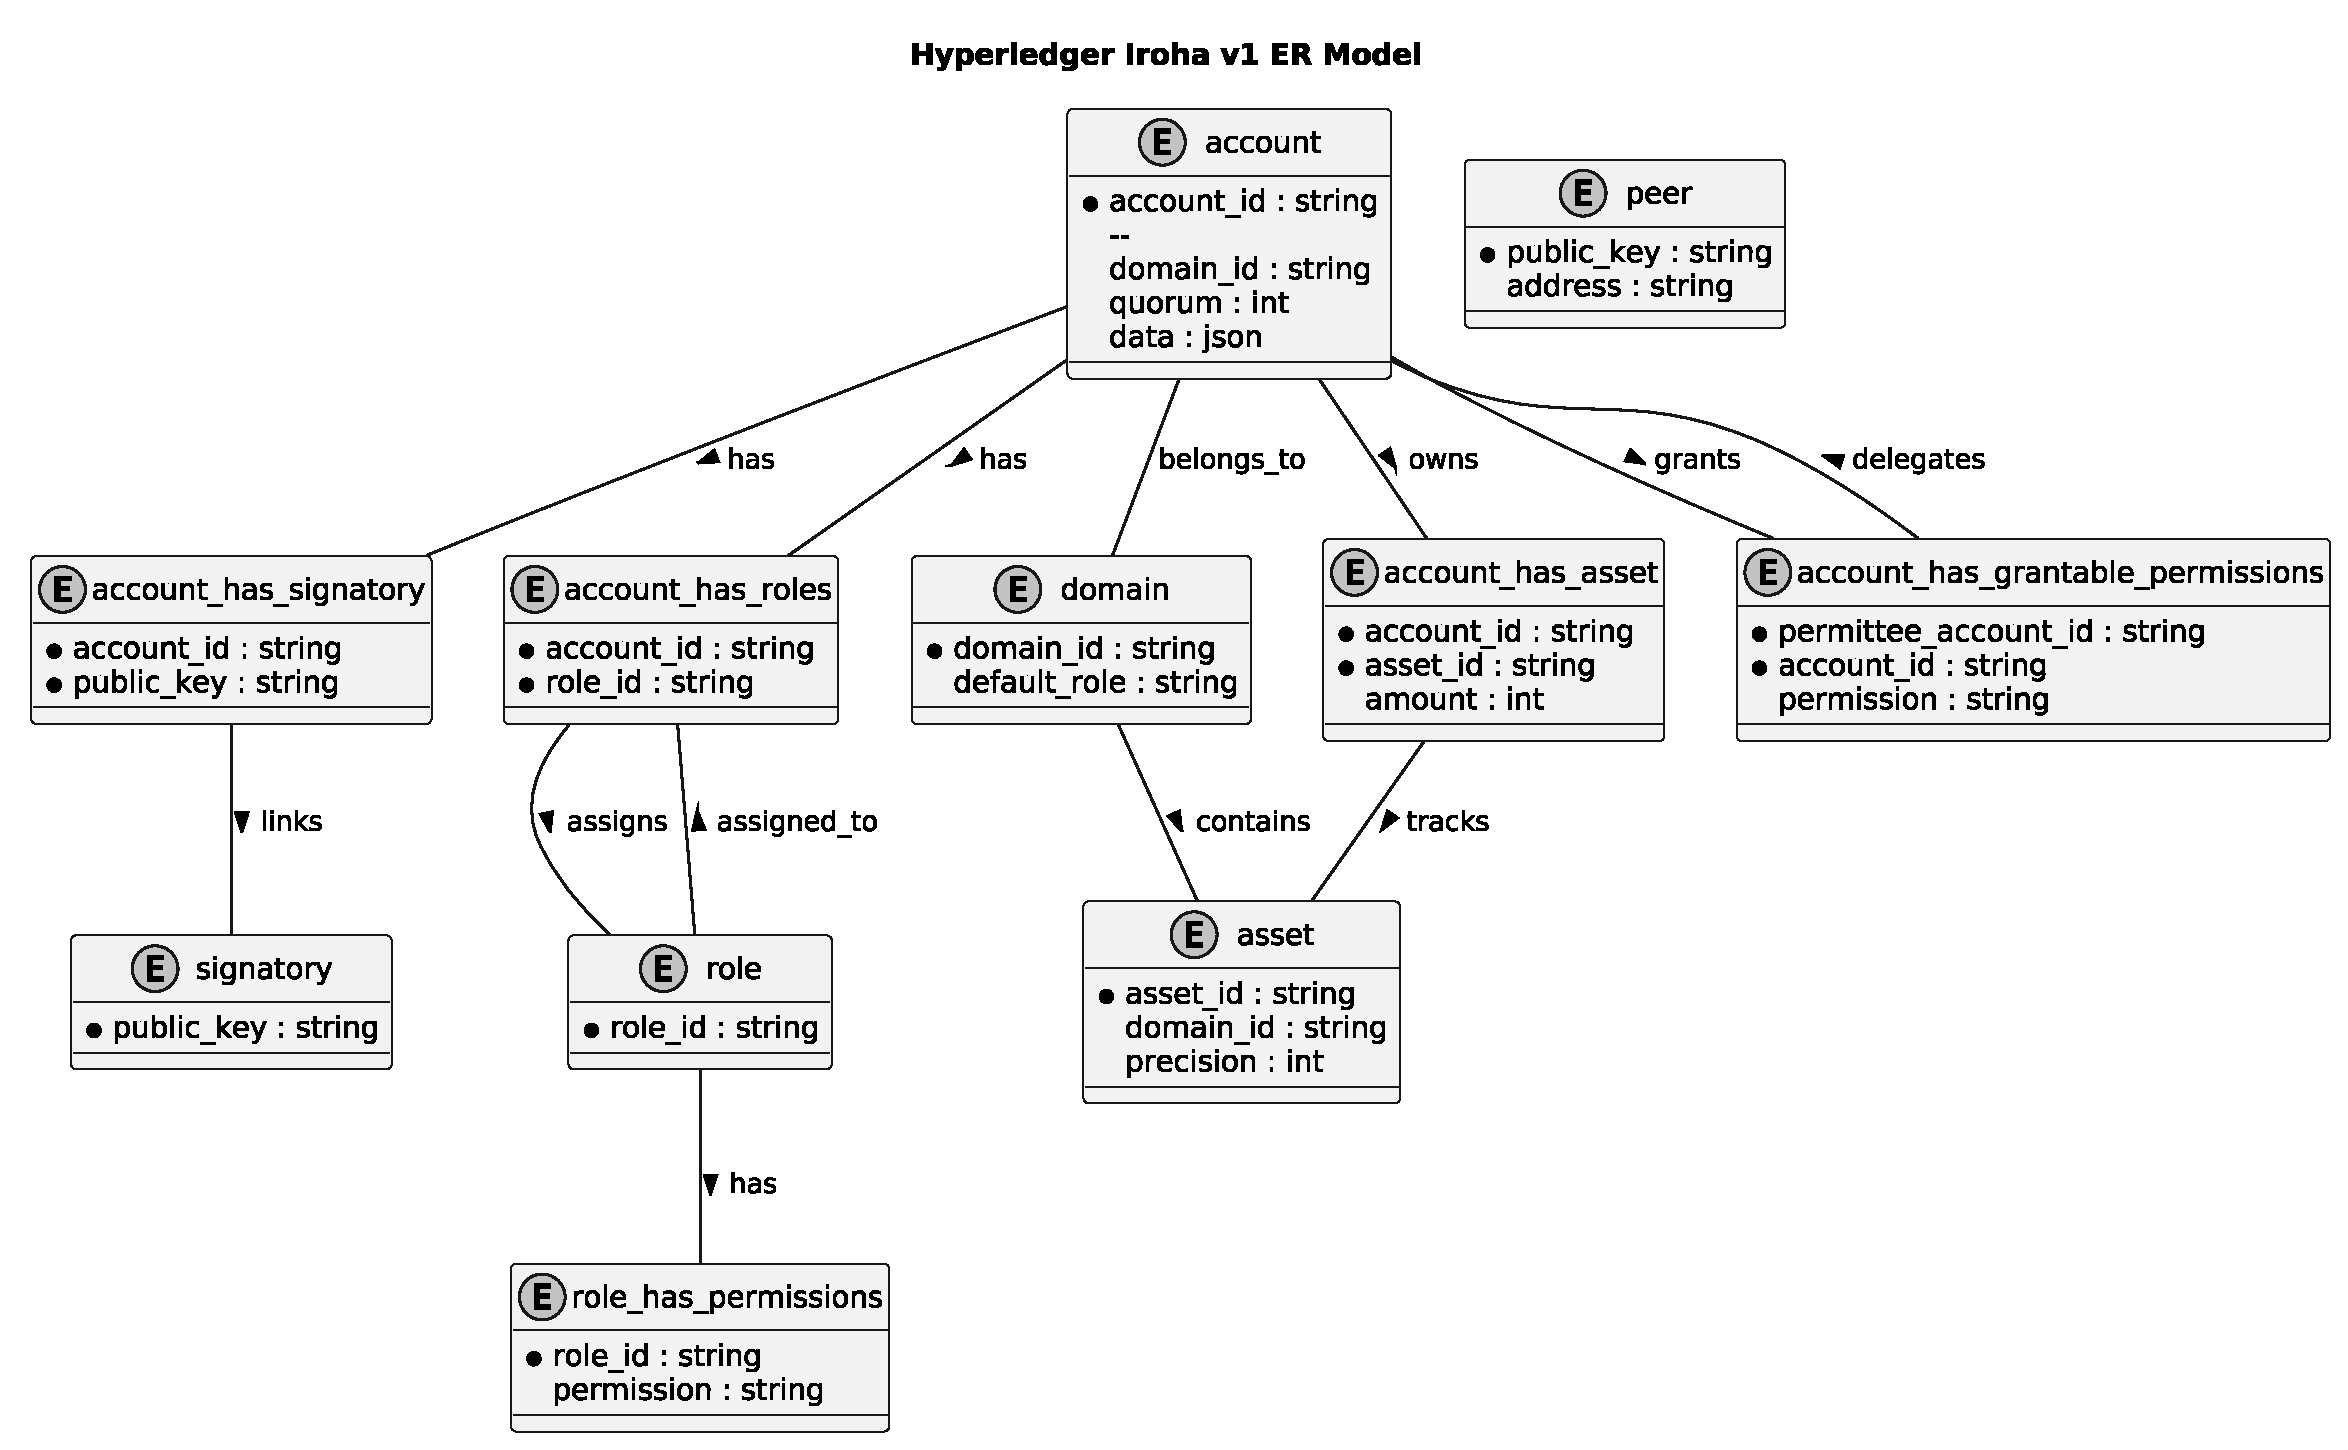
\includegraphics[width=0.98\textwidth, keepaspectratio]{iroha_v1_er_model.eps}
      \caption{Subset of the Iroha v1 Entity-relationship model}
      \label{fig:iroha_v1_er_model}
\end{figure}


This ER model follows Hyperledger Iroha’s permissioned blockchain structure. It ensures fine-grained access control, multi-signature security, and domain-based account management.


\subsection{Relationship Between the Open Science Platform ER Model and the Iroha v1 ER Model}

The Open Science Platform ER model leverages the entity structure of the Iroha v1 ER model, particularly the \texttt{account} entity, to represent both the \texttt{User} and \texttt{Project} entities. In this approach, instead of introducing separate entitties for users and projects, the \texttt{account} entity in the Iroha v1 ER model serves as a general-purpose representation, encapsulating all necessary attributes in a structured format.

The attributes specific to users and projects, which are not natively present in the Iroha v1 \texttt{account} entity, are stored as JSON objects within the \texttt{data} field of the \texttt{account} entity. This design provides a flexible and scalable means of extending the entity's attributes without modifying the core schema of the Iroha blockchain.

From a relational perspective, the \texttt{account} entity maintains its standard associations with roles, permissions, and assets as defined in the Iroha v1 ER model. This ensures that user accounts and project accounts can both participate in the blockchain's permissioning system, asset ownership model, and role-based access control without requiring modifications to the underlying structure.

By reusing the \texttt{account} entity, the Open Science Platform ER model ensures compatibility with Iroha's existing mechanisms for identity management, cryptographic signing, and permission delegation. Additionally, this approach aligns with the decentralized and immutable nature of blockchain, ensuring that both user and project entities benefit from the security and transparency features inherent to the Iroha v1 framework.



\begin{figure}[htbp]
      \centering
      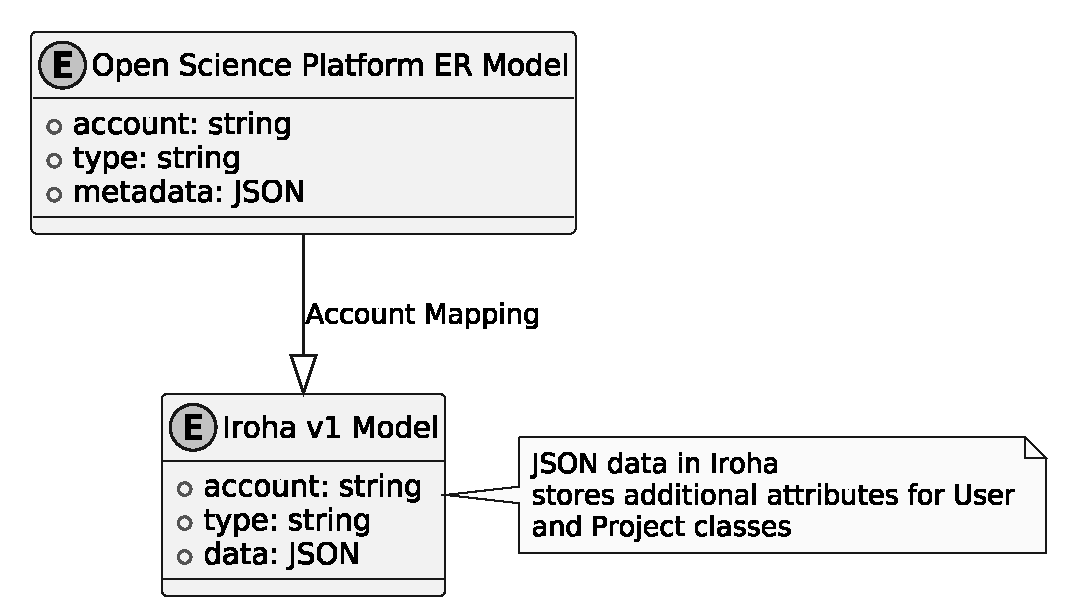
\includegraphics[width=0.98\textwidth, keepaspectratio]{comparing_er_models.eps}
      \caption{Comparison of the Entintiy-relationship models}
      \label{fig:comparing_er_models}
\end{figure}


\subsection{The role of metadata and ontologies in the Open Science Platform}

Metadata plays a crucial role in both the \texttt{Account} and \texttt{Project} classes within the Open Science platform. It is used to capture and represent essential information about the user and the research project, providing context and structure to their respective data. This metadata is stored in JSON format, following established semantic web standards and leveraging ontologies to enhance data interoperability and accessibility.


\subsection{Selected Ontologies}
An ontology is a formal representation of knowledge as a set of concepts within a domain and the relationships between those concepts. In the context of the Open Science platform, ontologies help structure data in a way that promotes interoperability, consistency, and clarity. The use of ontologies such as \texttt{FOAF}, \texttt{Schema.org}, and \texttt{Dublin Core} ensures that data is standardized and can be easily shared and understood across different systems.

\begin{table}[h]
      \centering
      \label{tab:ontologies}
      \renewcommand{\arraystretch}{1.2}
      \begin{tabularx}{\textwidth}{|l|X|}            \hline
            \textbf{Ontology}                  & \textbf{Description}                                                                                                                                                                                                                                   \\ \hline
            \textbf{FOAF (Friend of a Friend)} & A vocabulary used to describe people, their activities, and their relationships to other people and objects. It is used to describe the \texttt{User} entity, including attributes like name, email, and organization.                                 \\ \hline
            \textbf{Schema.org}                & A collaborative initiative that provides a structured vocabulary for data markup on the web. It is used for describing both \texttt{User} and \texttt{Project} metadata, ensuring compatibility with web standards and promoting data discoverability. \\ \hline
            \textbf{Dublin Core (DC)}          & A metadata standard used for describing a wide range of resources, for describing the abstract, keywords, and other descriptive elements of the \texttt{Project} entity.                                                                               \\ \hline
      \end{tabularx}
      \caption{Ontologies used in the Open Science Platform}
\end{table}

These ontologies were chosen because of their widespread adoption, their ability to standardize data across different systems, and their support for rich, machine-readable representations. By aligning with these ontologies, the platform ensures that its metadata is compatible with other Open Science initiatives and services, facilitating seamless integration and data exchange.


\subsection{User Metadata}
The metadata for the \texttt{Account} class describes the attributes associated with a user on the platform. This metadata is structured using multiple ontologies, primarily \texttt{FOAF} (Friend of a Friend) and \texttt{Schema.org}, to provide detailed and interoperable information about the user. The key attributes in the \texttt{Account} metadata include the user's name, email, organizational affiliation, unique identifier (ORCID), role, public key, and linked project.

\begin{table}[h]
      \centering
      \label{tab:user_metadata}
      \renewcommand{\arraystretch}{1.2}
      \begin{tabularx}{\textwidth}{|l|X|}
            \hline
            \textbf{Attribute}              & \textbf{Description}                                                                                            \\ \hline
            \texttt{foaf:name}              & The name of the user.                                                                                           \\ \hline
            \texttt{foaf:mbox}              & The email address of the user.                                                                                  \\ \hline
            \texttt{foaf:organization}      & The organization the user is affiliated with, described as an instance of the \texttt{foaf:Organization} class. \\ \hline
            \texttt{schema:identifier}      & A unique identifier for the user, such as an ORCID identifier.                                                  \\ \hline
            \texttt{foaf:holdsAccount}      & The user's account details, including their role and public key.                                                \\ \hline
            \texttt{schema:linked\_project} & The project associated with the user.                                                                           \\ \hline
      \end{tabularx}
      \caption{Account Metadata Attributes}
\end{table}


\subsection{The use of JSON-LD for metadata representation}

JSON for Linked Data (JSON-LD) is a lightweight Linked Data format designed to structure and interconnect data on the web using standard JSON. It extends JSON by incorporating semantic web principles, making data more discoverable, reusable, and machine-readable. JSON-LD achieves this by including a \texttt{@context} element, which maps terms to well-defined ontologies, and a \texttt{@graph} element, which structures entities and their relationships in a linked data format.

A key advantage of JSON-LD is its compatibility with existing JSON-based systems while enabling seamless integration with the semantic web. By leveraging vocabularies such as Schema.org and Dublin Core, JSON-LD ensures interoperability across diverse platforms and datasets. This makes it particularly useful for Open Science applications, where structured metadata enhances research reproducibility and data sharing.

In the context of the Open Science platform, JSON-LD is used to encode metadata for users and research projects, ensuring alignment with widely accepted ontologies. The structured representation enables automatic indexing, metadata enrichment, and semantic search capabilities, facilitating better knowledge discovery and integration within the scientific community.


\subsection{The \texttt{User} Metadata JSON-LD object}

The user metadata is structured using two primary ontologies: Friend of a Friend (FOAF) and Schema.org.

The FOAF ontology is used to describe personal and organizational attributes of users within the platform. It provides well-defined properties such as \texttt{foaf:name} for the user’s full name, \texttt{foaf:mbox} for email addresses, and \texttt{foaf:organization} for institutional affiliations. By leveraging FOAF, the platform ensures standardized representation of user identities and their associations, facilitating integration with other systems that utilize FOAF-based user profiles.

Schema.org complements FOAF by enriching the user metadata with structured properties that enhance discoverability and machine readability. The \texttt{schema:identifier} property, for instance, is used to store unique user identifiers such as ORCID, ensuring compatibility with global researcher identification systems. Additionally, \texttt{schema:roleName} captures the user’s role within the platform (e.g., reviewer, publisher), while \texttt{schema:publicKey} stores cryptographic keys associated with the user’s account. The \texttt{schema:linked\_project} property establishes connections between users and their associated research projects, enabling efficient metadata retrieval and knowledge graph construction as exhibited in Figure~\ref{jsonld:user}, the JSON-LD structure represents the project metadata in the Open Science platform.



\begin{figure}[h]
      \centering
      \caption{JSON-LD structure for user metadata in the Open Science platform}
      \label{jsonld:user}
      \begin{verbatim}
  {
      "@context": {
          "schema": "http://schema.org/",
          "foaf": "http://xmlns.com/foaf/0.1/"
      },
      "@graph": [
          {
              "@type": "foaf:Person",
              "foaf:name": "Zealous Ptolemy",
              "foaf:mbox": "zealous_ptolemy@email.com",
              "foaf:organization": {
                  "@type": "foaf:Organization",
                  "foaf:name": "Ashkelon Academic College"
              },
              "schema:identifier": {
                  "@type": "PropertyValue",
                  "propertyID": "ORCID",
                  "value": "6153-7096-0437-X"
              },
              "foaf:holdsAccount": {
                  "schema:identifier": "zealous_ptolemy@test",
                  "schema:roleName": "reviewer",
                  "schema:publicKey": "ca4c00c0a43bbd2caf070ab780886906ebb70e2c3d975972ccab4e15c01f33bd"
              },
              "schema:linked_project": "02226@test"
          }
      ]
  }
  \end{verbatim}
\end{figure}



By combining FOAF and Schema.org, the Open Science platform ensures that user metadata is both human-readable and machine-actionable, promoting seamless integration with external research infrastructures and fostering an interoperable ecosystem for Open Science.

\subsection{The \texttt{Project} Metadata JSON-LD object}

The metadata for the \texttt{Project} entity provides essential details about the research project hosted on the platform. Similar to the user metadata, the project metadata is structured using \texttt{Schema.org} and \texttt{Dublin Core} (\texttt{dc}) ontologies. This structure allows for a comprehensive description of the project, including its name, abstract, keywords, timeline, funding details, and location.

\begin{table}[h]
      \centering
      \label{tab:project_metadata}
      \renewcommand{\arraystretch}{1.2}
      \begin{tabularx}{\textwidth}{|l|X|}
            \hline
            \textbf{Attribute}           & \textbf{Description}                                                                                           \\ \hline
            \texttt{schema:name}         & The name of the research project.                                                                              \\ \hline
            \texttt{dc:abstract}         & A brief abstract describing the project's objectives and focus.                                                \\ \hline
            \texttt{schema:keywords}     & Keywords associated with the project, such as "precision agriculture" and "global supply chains."              \\ \hline
            \texttt{schema:startDate}    & The start date of the project.                                                                                 \\ \hline
            \texttt{schema:endDate}      & The end date of the project.                                                                                   \\ \hline
            \texttt{schema:funding}      & The funding organization for the project, described as an instance of the \texttt{schema:Organization} class.  \\ \hline
            \texttt{schema:location}     & The physical location where the project is based, described as an instance of the \texttt{schema:Place} class. \\ \hline
            \texttt{schema:metadataCID}  & A unique identifier for the metadata of the project.                                                           \\ \hline
            \texttt{schema:linked\_user} & The user associated with the project.                                                                          \\ \hline
      \end{tabularx}
      \caption{Project Metadata Attributes}
\end{table}

The following JSON structure describes the metadata for a \texttt{Project} in the Open Science platform as shown in Figure~\ref{jsonld:project}.


\begin{figure}[h]
      \centering
      \caption{JSON-LD structure for project metadata in the Open Science platform}
      \label{jsonld:project}
      \begin{verbatim}
  {
      "@context": {
          "schema": "http://schema.org/",
          "dc": "http://purl.org/dc/terms/"
      },
      "@graph": [
          {
              "@type": "schema:ResearchProject",
              "schema:identifier": "02226@test",
              "schema:publicKey": "1c6b8d00c8382c93eb0dd3eeb24a20bfece56a28326bbaebb647cadaf4750520",
              "schema:description": {
                  "@context": {
                      "schema": "http://schema.org/",
                      "dc": "http://purl.org/dc/terms/"
                  },
                  "@type": "schema:ResearchProject",
                  "schema:name": "Assessing the Benefits of precision agriculture for global supply chains",
                  "dc:abstract": "This research focuses on the benefits and challenges posed by precision agriculture for global supply chains, with an emphasis on its potential for disease prevention.",
                  "schema:keywords": [
                      "precision agriculture",
                      "global supply chains",
                      "disease prevention"
                  ],
                  "schema:startDate": "2023-12-18",
                  "schema:endDate": "2027-01-02",
                  "schema:funding": {
                      "@type": "schema:Organization",
                      "schema:name": "World Wildlife Fund"
                  },
                  "schema:location": {
                      "@type": "schema:Place",
                      "schema:name": "Los Angeles, California, USA"
                  }
              },
              "schema:metadataCID": "Qmay4cDaxUaZaHoJKqzN69XkiX8wMx17aG4VMmwmkLcL1a",
              "schema:linked_user": "zealous_ptolemy@test"
          }
      ]
  }
  \end{verbatim}
\end{figure}


This metadata not only captures the essential details of the project but also ensures that these details are linked to the user's profile, making it easier to track the relationship between users and their associated research efforts.


\subsection{General Metadata Handling Workflow}

The Open Science platform follows a general approach to metadata handling, ensuring that it is properly formatted, stored, and made immutable through blockchain integration. The process begins with processing the relevant metadata, which may pertain to a user, project, or file. This metadata is then formatted according to the JSON-LD standard, ensuring semantic interoperability and alignment with established ontologies.

Once formatted, the JSON-LD object is sent to the InterPlanetary File System (IPFS), a decentralized storage solution that provides content-addressable storage. Upon successful storage, IPFS generates a unique Content Identifier (CID) that serves as a reference to the stored metadata. This CID is then recorded on the blockchain by writing it into the account details associated with the entity. By anchoring the metadata CID on the blockchain, the platform ensures integrity, immutability, and transparency.

Finally, the blockchain transaction containing the CID serves as a provenance record, allowing stakeholders to verify and trace metadata modifications over time. The entire workflow guarantees that metadata remains both accessible and verifiable, promoting reproducibility and trust within the Open Science ecosystem.

Figure~\ref{fig:metadata_workflow} illustrates the sequence of operations in the metadata handling process.


\begin{figure}[htbp]
      \centering
      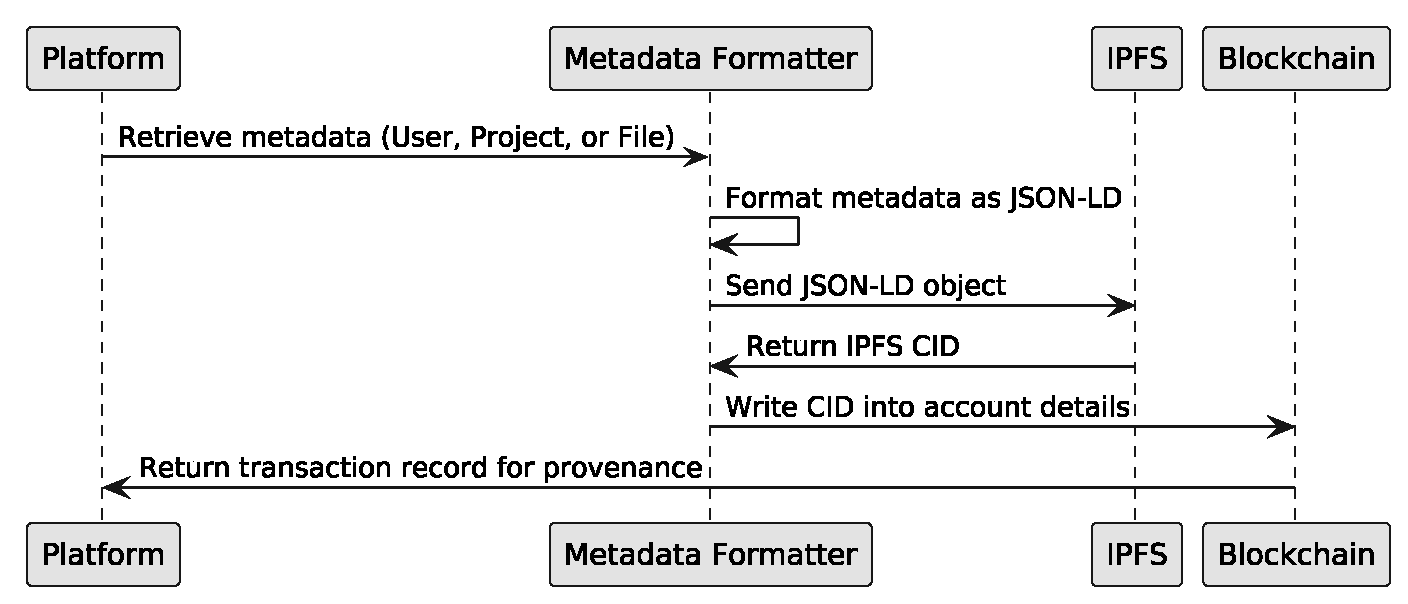
\includegraphics[width=0.98\textwidth, keepaspectratio]{metadata_workflow_sequence.eps}
      \caption{General workflow for metadata handling in the Open Science Platform}
      \label{fig:metadata_workflow}
\end{figure}

\subsection{Blockchain Representation of Metadata}

In the Open Science platform, metadata for users, projects, and files are stored on the blockchain. This ensures the integrity and provenance of the metadata while leveraging decentralized technologies. The following subsections describe the structure of blockchain representations for both user and project data, as well as the files associated with these projects.

\subsection{User Account}

The representation of a user's account on the blockchain contains the standard Iroha v1 attributes for the account entity, such as the unique account identifier, domain information, and quorum for consensus. Additionally, the \texttt{json\_data} attribute references both the project to which the user is linked and the user's metadata CID (Content Identifier) stored on IPFS. This blockchain-based approach ensures that the user’s information remains immutable and traceable, which is critical for maintaining the integrity of research data.

The JSON structure describes the account details for a user in the Open Science platform as shown in Figure~\ref{fig:user_blockchain_representation}.

\begin{figure}[h]
      \centering
      \caption{Blockchain Representation of User Account}
      \label{fig:user_blockchain_representation}
      \begin{verbatim}
    {
        "account_id": "zealous_ptolemy@test",
        "domain_id": "test",
        "quorum": 1,
        "json_data": {
            "admin@test": {
                "linked_project": "02226@test",
                "account_metadata_cid": "QmT31fzDBNYAz1jAoAa7gQqSP7mDquv3fR8z1xLfxeHR5o"
            }
        }
    }
    \end{verbatim}
\end{figure}

\subsection{Project Account}

The project account representation similarly uses a blockchain-based structure to store project-related metadata. Each project is identified by a unique account ID, along with the project’s domain and quorum. The project metadata is linked to the user and includes important information about files associated with the project, including their CID references on IPFS. This ensures that the project data is linked to the user’s account and that all files and metadata related to the project are securely stored on the blockchain for provenance tracking.

The JSON structure describes the account details for a user in the Open Science platform as shown in Figure~\ref{fig:project_blockchain_representation}.


\begin{figure}[h]
      \centering
      \caption{Blockchain Representation of Project Account}
      \label{fig:project_blockchain_representation}
      \begin{verbatim}
    {
        "account_id": "02226@test",
        "domain_id": "test",
        "quorum": 1,
        "json_data": {
            "admin@test": {
                "file_1": [
                    "QmTLZSqzPexwEdniZXLPN6fUfmEXX6MXS3b4QjKURgxc9y",
                    "Qmchg7At5whR1T4xP8TwTMd8ntQqJXbbSicJRtGGaW1Z2P"
                ],
                "linked_user": "zealous_ptolemy@test",
                "account_metadata_cid": "Qmay4cDaxUaZaHoJKqzN69XkiX8wMx17aG4VMmwmkLcL1a"
            }
        }
    }
    \end{verbatim}
\end{figure}


\subsection*{File Representation}

Within the project account, each file associated with the project is represented by a CID pair. The first CID refers to the file stored on IPFS, while the second CID references the metadata associated with that file. This structure ensures that the file's content and its metadata are both stored and tracked independently, but are still linked to the blockchain for integrity and provenance.

\begin{itemize}
      \item The \textbf{first CID} (\texttt{QmTLZSqzPexwEdniZXLPN6fUfmEXX6MXS3b4QjKURgxc9y}) corresponds to the \textbf{file}.
      \item The \textbf{second CID} (\texttt{Qmchg7At5whR1T4xP8TwTMd8ntQqJXbbSicJRtGGaW1Z2P}) corresponds to the \textbf{metadata of the file}, ensuring that all relevant details are retrievable.
\end{itemize}

This structure allows for the efficient tracking and retrieval of research project data while maintaining provenance and integrity through blockchain storage.

\subsection{Provenance in the Open Science Platform}

The provenance system takes a two-fold approach, with both methods being native features of their respective systems. The first approach leverages Iroha v1’s transaction logging capabilities, where each transaction is recorded with a hexadecimal hash and timestamp. This provides a reliable mechanism for tracking the evolution of account states over time. The hash acts as a snapshot, allowing for the retrieval of any past state of an account based on the corresponding transaction hash.

The second approach makes use of IPFS’s native feature of Content Identifiers (CIDs) to track metadata associated with accounts, projects, and files. Each piece of metadata is linked to a unique CID, which allows for decentralized storage and immutability. A mismatch of the CID indicates that the metadata or file has been modified, ensuring the integrity of the information over time.

Together, these two approaches—transaction logging through Iroha v1’s blockchain and metadata tracking through IPFS CIDs—provide a robust and transparent provenance system, ensuring both the transaction history and the integrity of metadata are verifiably recorded and traceable.





\subsection{Smart Contract}

The platform deploys standard Ethereum EVM contracts in Solidity for account creation and detail setting. These contracts are deployed through the Iroha v1 Python Library.

\subsection{Benefits}

The Open Science platform offers numerous benefits for researchers and members of the scientific community, including:

\begin{itemize}
      \item Secure data sharing: By utilizing blockchain technology and IPFS, the platform ensures tamper-proof data exchange.
      \item Transparent data management: The use of smart contracts and decentralized storage guarantees transparency in data access and modification history.
      \item Collaborative research environment: The platform enables researchers to collaborate on projects, share artifacts and results, and track progress.
\end{itemize}

\subsection{Challenges}

The Open Science platform faces several challenges, including:

\begin{itemize}
      \item Scalability: As the number of users increases, the platform needs to be able to handle a growing amount of data and transactions efficiently.
      \item Interoperability: Ensuring seamless integration with existing research platforms and tools is crucial for widespread adoption.
      \item User Adoption: Educating researchers about the benefits of decentralized technologies and the Open Science platform can be an uphill battle.
\end{itemize}

\subsection{Future Work}

The Open Science platform has several areas for future development, including:

\begin{itemize}
      \item Integration with existing research platforms: Collaborations with established research platforms to expand the platform's reach and user base.
      \item Enhanced security measures: Implementing additional security protocols to protect against potential threats and maintain the integrity of shared information.
      \item User interface improvements: Enhancing the web interface to make it more user-friendly and accessible for researchers from diverse backgrounds.
\end{itemize}

\section{Conclusion}
The Open Science platform is a comprehensive solution for secure, transparent, traceable, and tamper-proof data sharing and collaboration. By leveraging decentralized technologies, the platform empowers researchers to share project artifacts and data in a reliable and trustworthy manner.

\end{document}



